\subsection{Motywacja}
Partycjonowanie siatek jest bardzo ważnym podproblemem dla wielu dziedzin.
Zastosowanie ma między innymi dla sieci komputerowych, także dla obliczeń równoległych, gdzie zależy nam,
aby problem podzielić na równe części pomiędzy węzły.
Jednym z takich problemów są symulacje $2$D.
Dla symulacji definiujemy zasady jej odbywania oraz siatkę, na której ma się odbywać.
Celem takiej symulacji może być przykładowo zbadanie ruchu pieszego na mapie galerii, następnie wyodrębnienie miejsc
zatłoczonych, które wymagają poprawek w projekcie.
Innym przykładem symulacji jest symulacja królików i kapusty przedstawiona na rysunku \ref{im:kroliki}.

Z racji na wielkość mapy często taka symulacja jest bardzo wymagająca obliczeniowo, dlatego dążymy do jej
zrównoleglenia.
Jedną z metod zrównoleglenia tego typu obliczeń jest podział siatki wejściowej pomiędzy węzły obliczeniowe,
tak by każdy węzeł zajmował się swoim obszarem.
Węzły mogą otrzymywać obszary równe w kwestii pola, jeśli są to węzły homogeniczne, lub obszary proporcjonalne do ich
możliwości obliczeniowych, jeśli są heterogeniczne.
Problemem, który towarzyszy tego typu zrównolegleniom jest narzut komunikacji.
Podzielone części siatki, tak naprawdę funkcjonują jako całość, węzły więc muszą wiedzieć co dzieje się na granicach u sąsiadów,
aby symulacja odbywała się prawidłowo.
Komunikacja pomiędzy węzłami rodzi więc dodatkowy narzut.
W celu zminimalizowania narzut komunikacyjnego należy więc zminimalizować długość granic pomiędzy obszarami.

\begin{figure}[h]
    \centering
    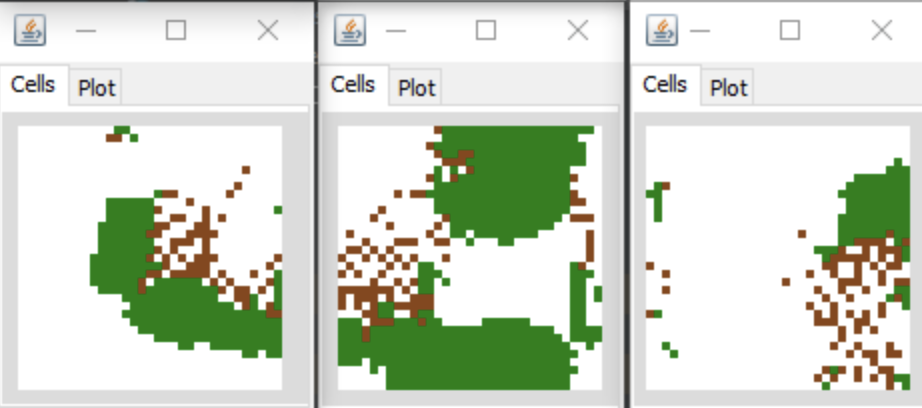
\includegraphics[width=0.6\linewidth]{images/kroliki}
    \caption{Fragment symulacja dla problemu królików i kapusty. Króliki zjadają kapustę zwiększając swoją populację. Ze względu
    na zwiększoną populację królików i spadającą liczbę pożywienia populacja królików spada, z czasem pozwalając
    populacji kapusty po raz kolejny się odrodzić. Każde okno obsługiwany jest przez osobny rdzeń procesora.}
    \label{im:kroliki}
\end{figure}

Patrząc na symulacje jak ta przedstawiona na rysunku \ref{im:kroliki}, łatwo zaproponować bardzo dobry podział, ponieważ
siatka jest prostokątna.
Podział otrzymamy rysując pionowe oraz poziomie separatory na siatce.
Jeśli przyjmiemy właściwy sposób ich rysowania otrzymamy idealny podział zarówno pod względem wielkości pól, jak i
długości granic pomiędzy obszarami.
Problem ten jednak przestaje być trywialny, jeśli siatka nie jest prostokątem lub chcemy, aby wyodrębnione obszary takiej
siatki nie zostały podzielone między partycje, to znaczy należały zawsze do jednej partycji.
Często również obliczenia z różnych powodów nigdy nie odbędą się na pewnych obszarach siatki.
Mogą być to na przykład ściany na mapie galerii lub też pomieszczenia, do których nie wchodzą klienci.
Chcemy aby tego typu obszary zostały również ujęte w podziale siatki, możemy bowiem wyobrazić sobie sytuację, że
jeden węzeł otrzymuje do symulowania część siatki właśnie z obszarem, na którym symulacja nie będzie się odbywać.
Nie będzie on wtedy wykorzystywany do symulacji.
